%!TEX root = ../thesis.tex
%*******************************************************************************
%****************************** Fifth Chapter **********************************
%*******************************************************************************
\chapter{Evaluation}\label{Evaluation}

% **************************** Define Graphics Path **************************
\ifpdf
    \graphicspath{{Chapter5/Figs/Raster/}{Chapter5/Figs/PDF/}{Chapter5/Figs/}}
\else
    \graphicspath{{Chapter5/Figs/Vector/}{Chapter5/Figs/}}
\fi

This chapter will evaluate the program's performance and results as the number of inputs scale. This chapter will also evaluate if the project was successful by comparison against the previously established objectives and requirements.

\section{Growth vs. Performance}
This section serves to test and evaluate the program's performance as it scales with the amount of nodes placed i.e. where the program and it's results become infeasible. This is important as it evaluates whether the program has been successful in it's effectiveness. These tests will be ran on the system described in Section \ref{sysinfo} and outlined in Appendix \ref{app:sysinfo}.

Each test will have a set amount of nodes, used to judge how the results and performance improve or degrade as the count of nodes increases. Each test performed will have an time limit, used to judge how the results improve as time increases. To ensure fairness, if two tests have the same node count: the same node layout will be used to ensure fair comparison between objective values.

\begin{landscape}
\begin{longtable}{r cc cc c c c c}
\caption{Test Case Parameters}\label{table:testcases} \\
\toprule
\multirow{2}{*}{Test Case} 
& \multicolumn{2}{c}{Building Node} 
& \multicolumn{2}{c}{Source Node} 
& \multirow{2}{*}{Time Limit (mins:secs)} 
& \multirow{2}{*}{Runtime (mins:secs)} 
& \multirow{2}{*}{Best Obj. Value} 
& \multirow{2}{*}{Figure Ref.} \\
\cmidrule(lr){2-3} \cmidrule(lr){4-5}
& Count & Pressure Req. & Count & Pressure Output & & & \\
\midrule
\endfirsthead

\multicolumn{9}{c}{{\bfseries \tablename\ \thetable{} -- continued from previous page}} \\
\toprule
\multirow{2}{*}{Test Case} 
& \multicolumn{2}{c}{Building Node} 
& \multicolumn{2}{c}{Source Node} 
& \multirow{2}{*}{Time Limit (mins:secs)}
& \multirow{2}{*}{Runtime (mins:secs)}
& \multirow{2}{*}{Best Obj. Value} 
& \multirow{2}{*}{Figure Ref.} \\
\cmidrule(lr){2-3} \cmidrule(lr){4-5}
& Count & Pressure Req. & Count & Pressure Output & & & \\
\midrule
\endhead

\midrule \multicolumn{9}{r}{{Continued on next page}} \\
\endfoot

\bottomrule
\endlastfoot

% Placeholder rows, replace with data if desired
1 & 3 & 1 & 1 & 3 & 10:00 & <0:01 & 70 & \ref{fig:testcase1results} \\
2 & 8 & 1 & 2 & 4 & 10:00 & 0:07 & 136 & \ref{fig:testcase2results} \\
3 & 20 & 1 & 5 & 4 & 10:00 & DNF & 312 & \ref{fig:testcase3results} \\
4 & 90 & 1 & 10 & 9 & 10:00 & DNF & 1042 & \ref{fig:testcase4results} \\
5 & 90 & 1 & 10 & 9 & 20:00 & DNF & 1011 & \ref{fig:testcase5results} \\

\end{longtable}
\end{landscape}


\subsection{Test Case One}
For this test case, the optimiser is very effective and found the optimal solution in $<1$ second.

\begin{figure}[H]
    \centering
    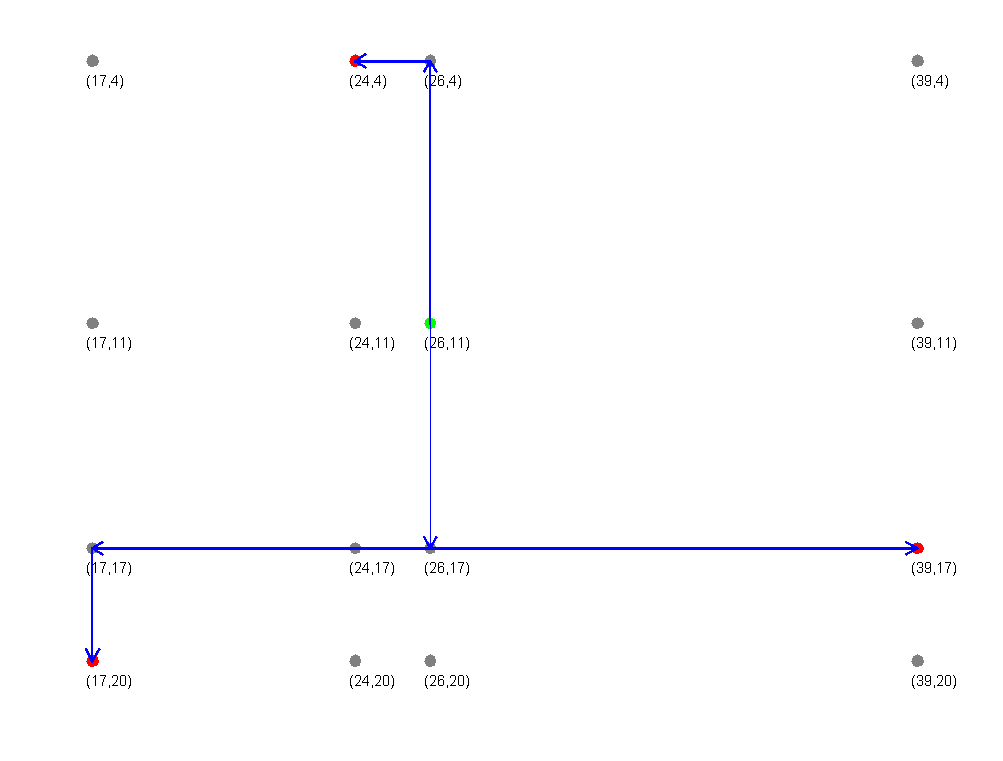
\includegraphics[width=1.0\linewidth]{resultstest2.png}
    \caption{The results of a test case involving four nodes}
    \label{fig:testcase1results}
\end{figure}

\subsection{Test Case Two}

\begin{figure}[H]
    \centering
    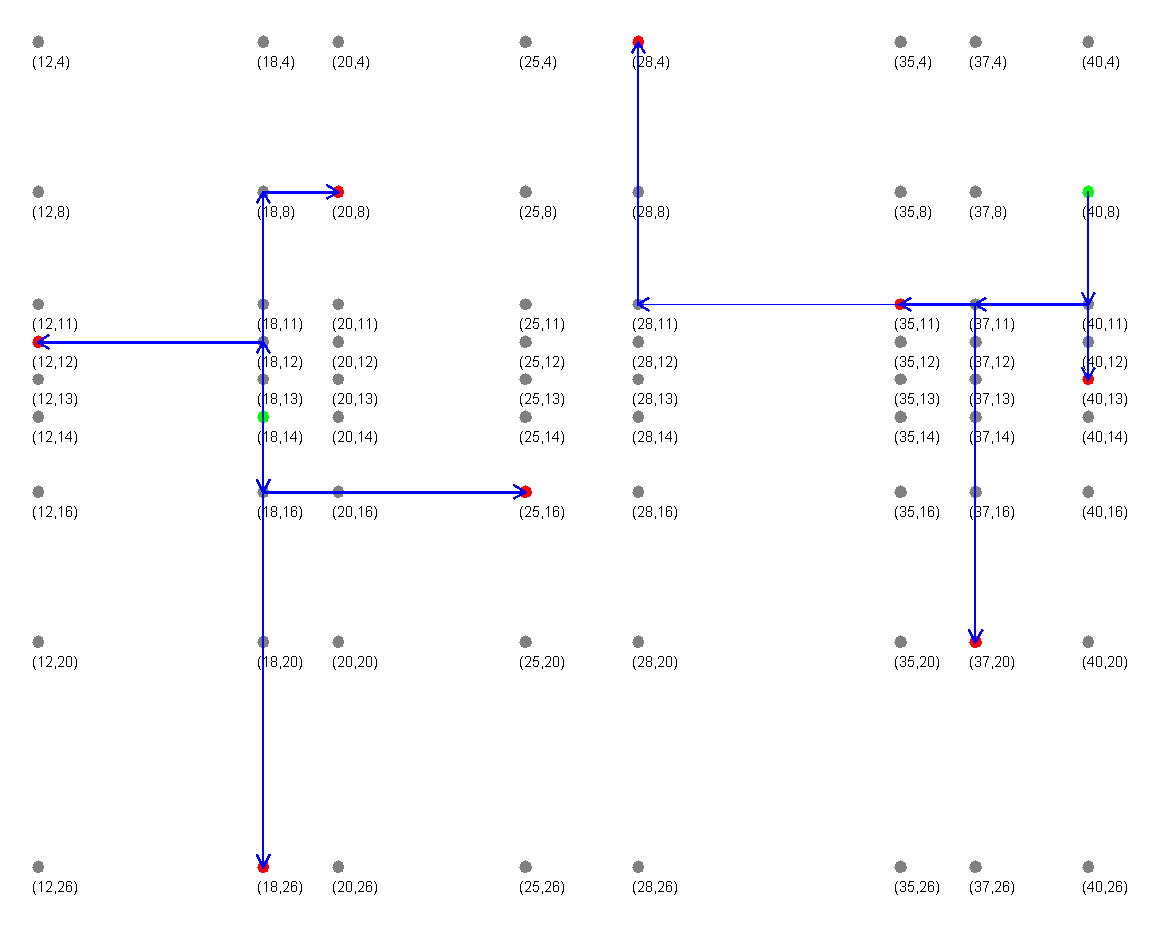
\includegraphics[width=0.9\linewidth]{resultstest3.png}
    \caption{The results of a test case involving ten nodes}
    \label{fig:testcase2results}
\end{figure}
For this test case, the optimiser was very effective once again and found the optimal solution in just seven seconds - a task that would ordinarily take significantly longer to find the optimal solution manually.

\subsection{Test Case Three}\label{testcase3}

\begin{figure}[H]
    \centering
    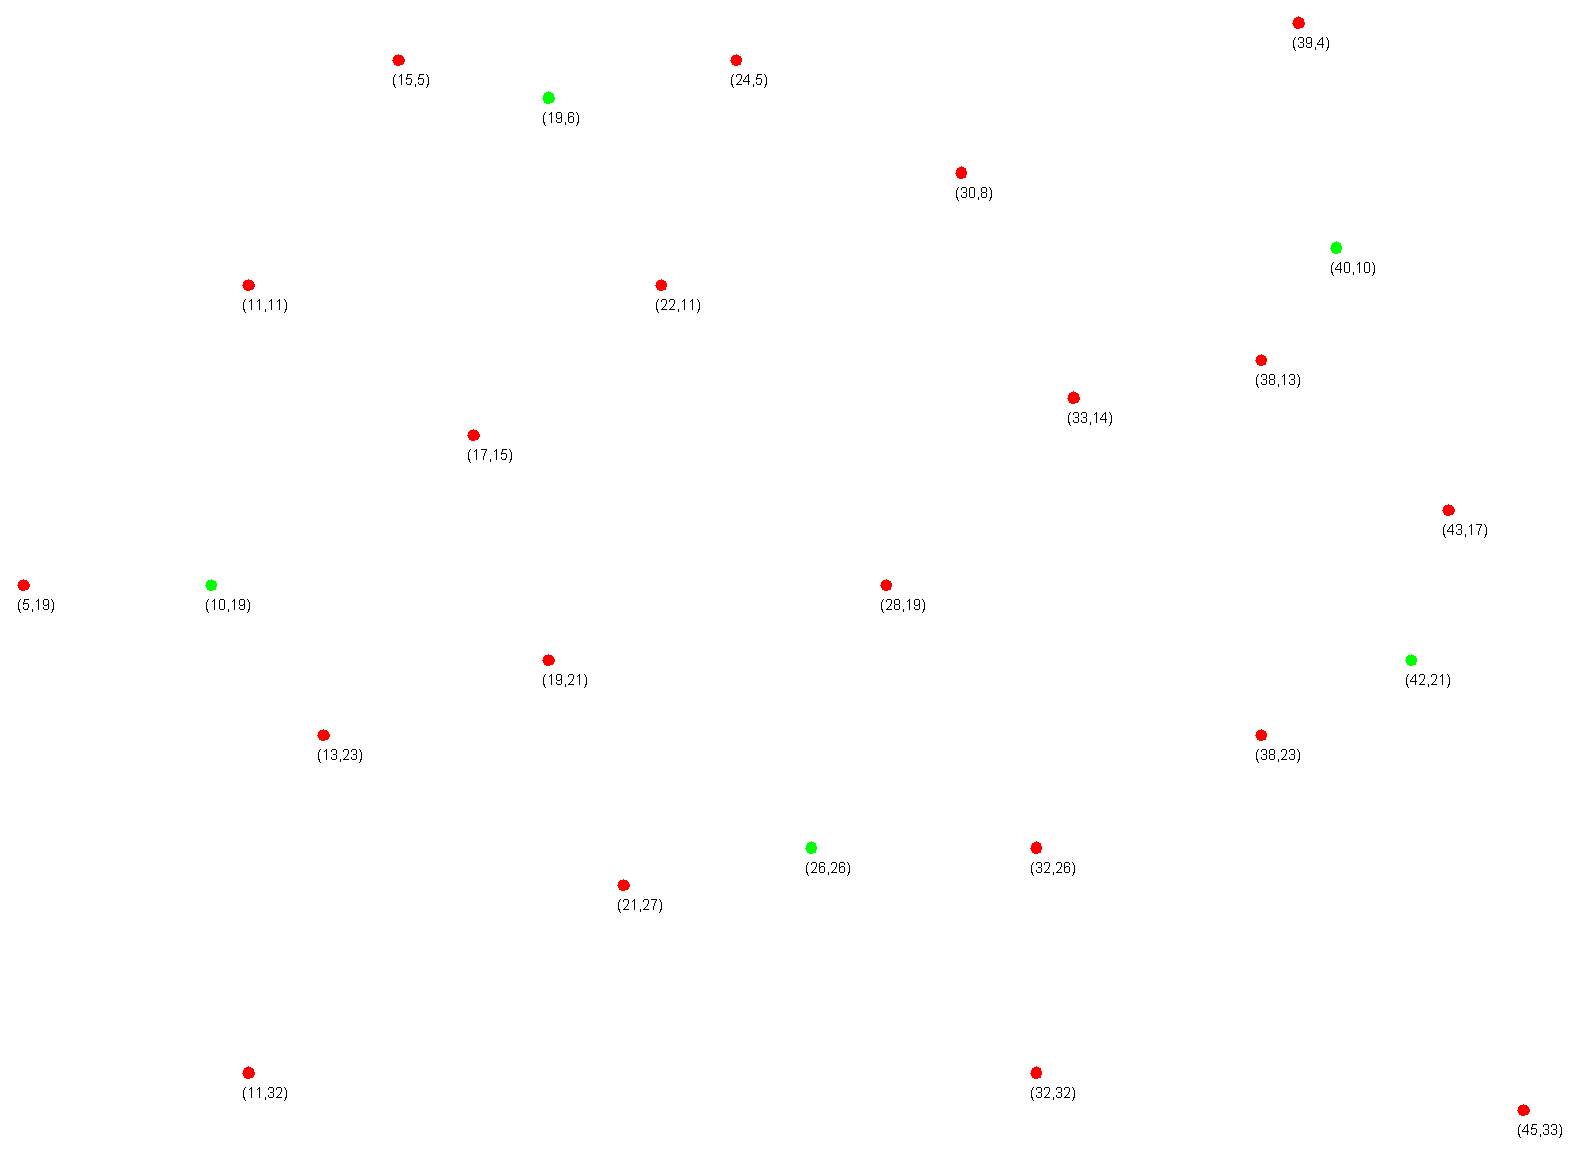
\includegraphics[width=0.9\linewidth]{test4.png}
    \caption{A test case involving twenty-five nodes}
    \label{fig:testcase3}
\end{figure}

In this case, the optimiser ran for the full ten minute limit and found the best objective value to be 312. However, the interesting note to make is that this conclusion was made a minute and seventeen seconds into the program's runtime. The remaining eight minutes spent trying to find a better solution did not succeed, a testament to the efficiency of the program. However a very viable - close to optimal - solution was still found in a time significantly quicker than could be manually achieved. More time would be required for the optimiser to complete in order to be confident this result was optimal. This indicates that as the input size increases, so does the necessary runtime for the program. 

\begin{figure}[H]
    \centering
    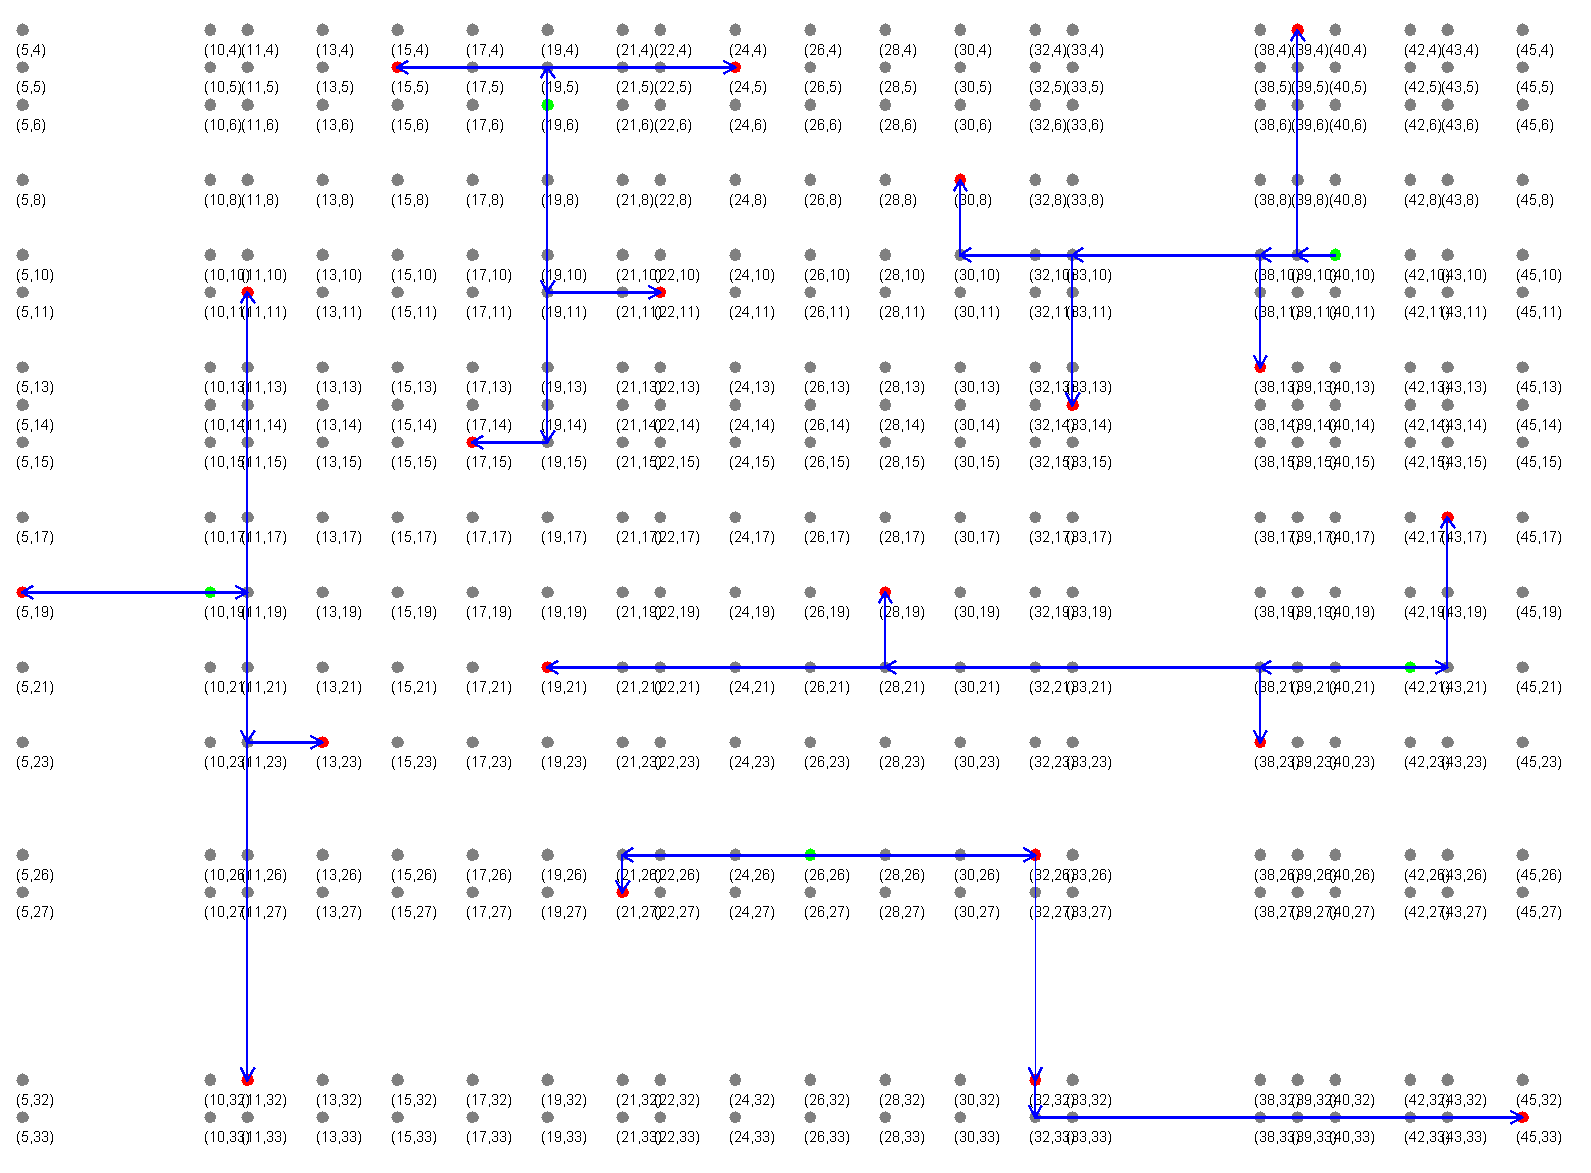
\includegraphics[width=0.9\linewidth]{resultstest4.png}
    \caption{The results of a test case involving twenty-five nodes}
    \label{fig:testcase3results}
\end{figure}

\subsection{Test Case Four}\label{testcase4}
The results are as follows:
\begin{figure}[H]
    \centering
    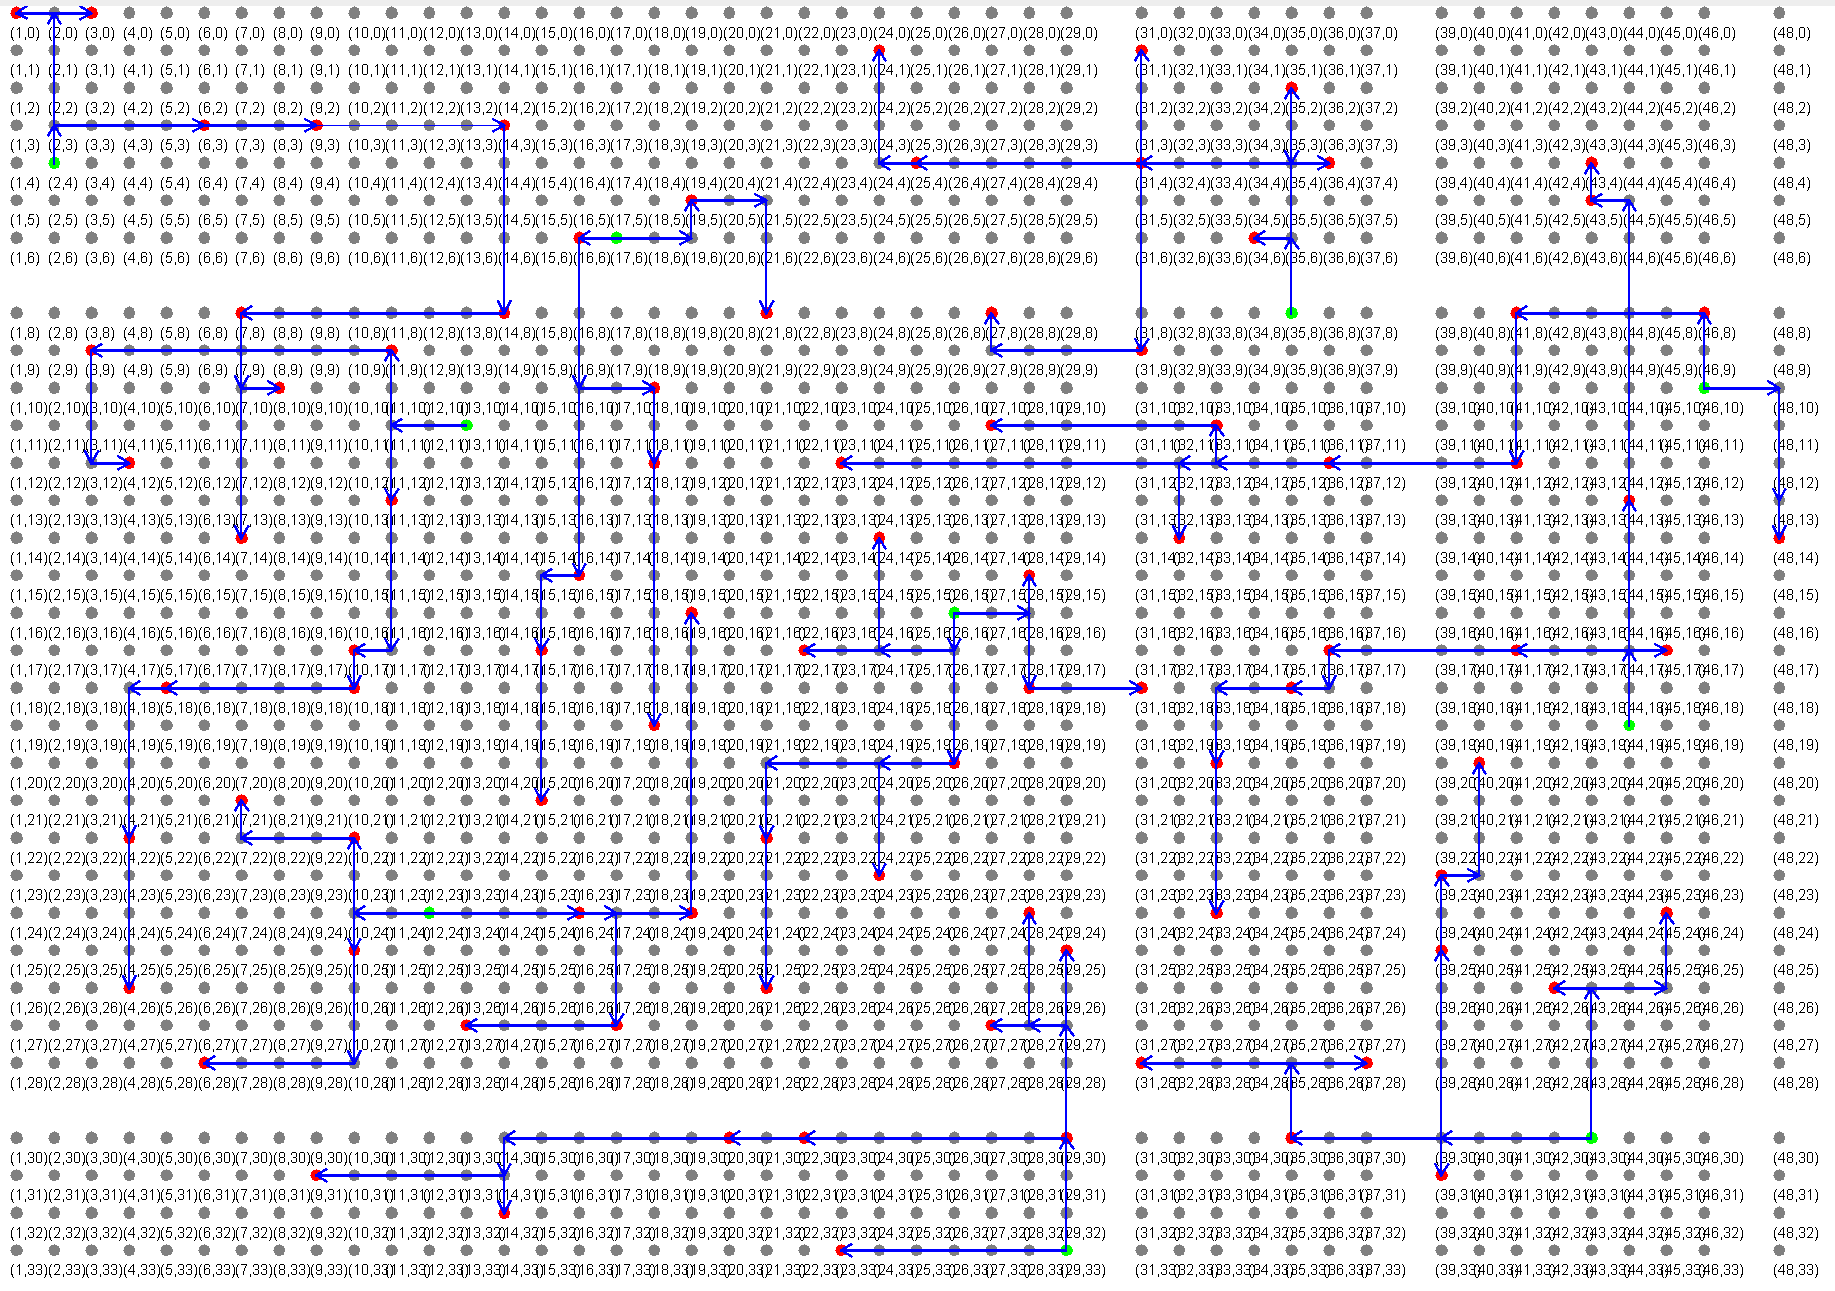
\includegraphics[width=0.9\linewidth]{resultstest5.png}
    \caption{The results of a test case involving a hundred nodes}
    \label{fig:testcase4results}
\end{figure}

This was the most illuminating of the test cases thus far. Once again, the program ran for the full allotted ten minutes. However in this case, unlike in Section \ref{testcase3}, better solutions were consistently found throughout the program's runtime, with the latest solution of 1042 found at eight minutes and fifty-seven seconds. This indicates there is potentially better solutions left undiscovered as a limitation of the runtime.

\subsection{Test Case Five}
Given the results described in Section \ref{testcase4}, it is important to allow the program to run longer to see if even more time may be required to find a better solution.

\begin{figure}[H]
    \centering
    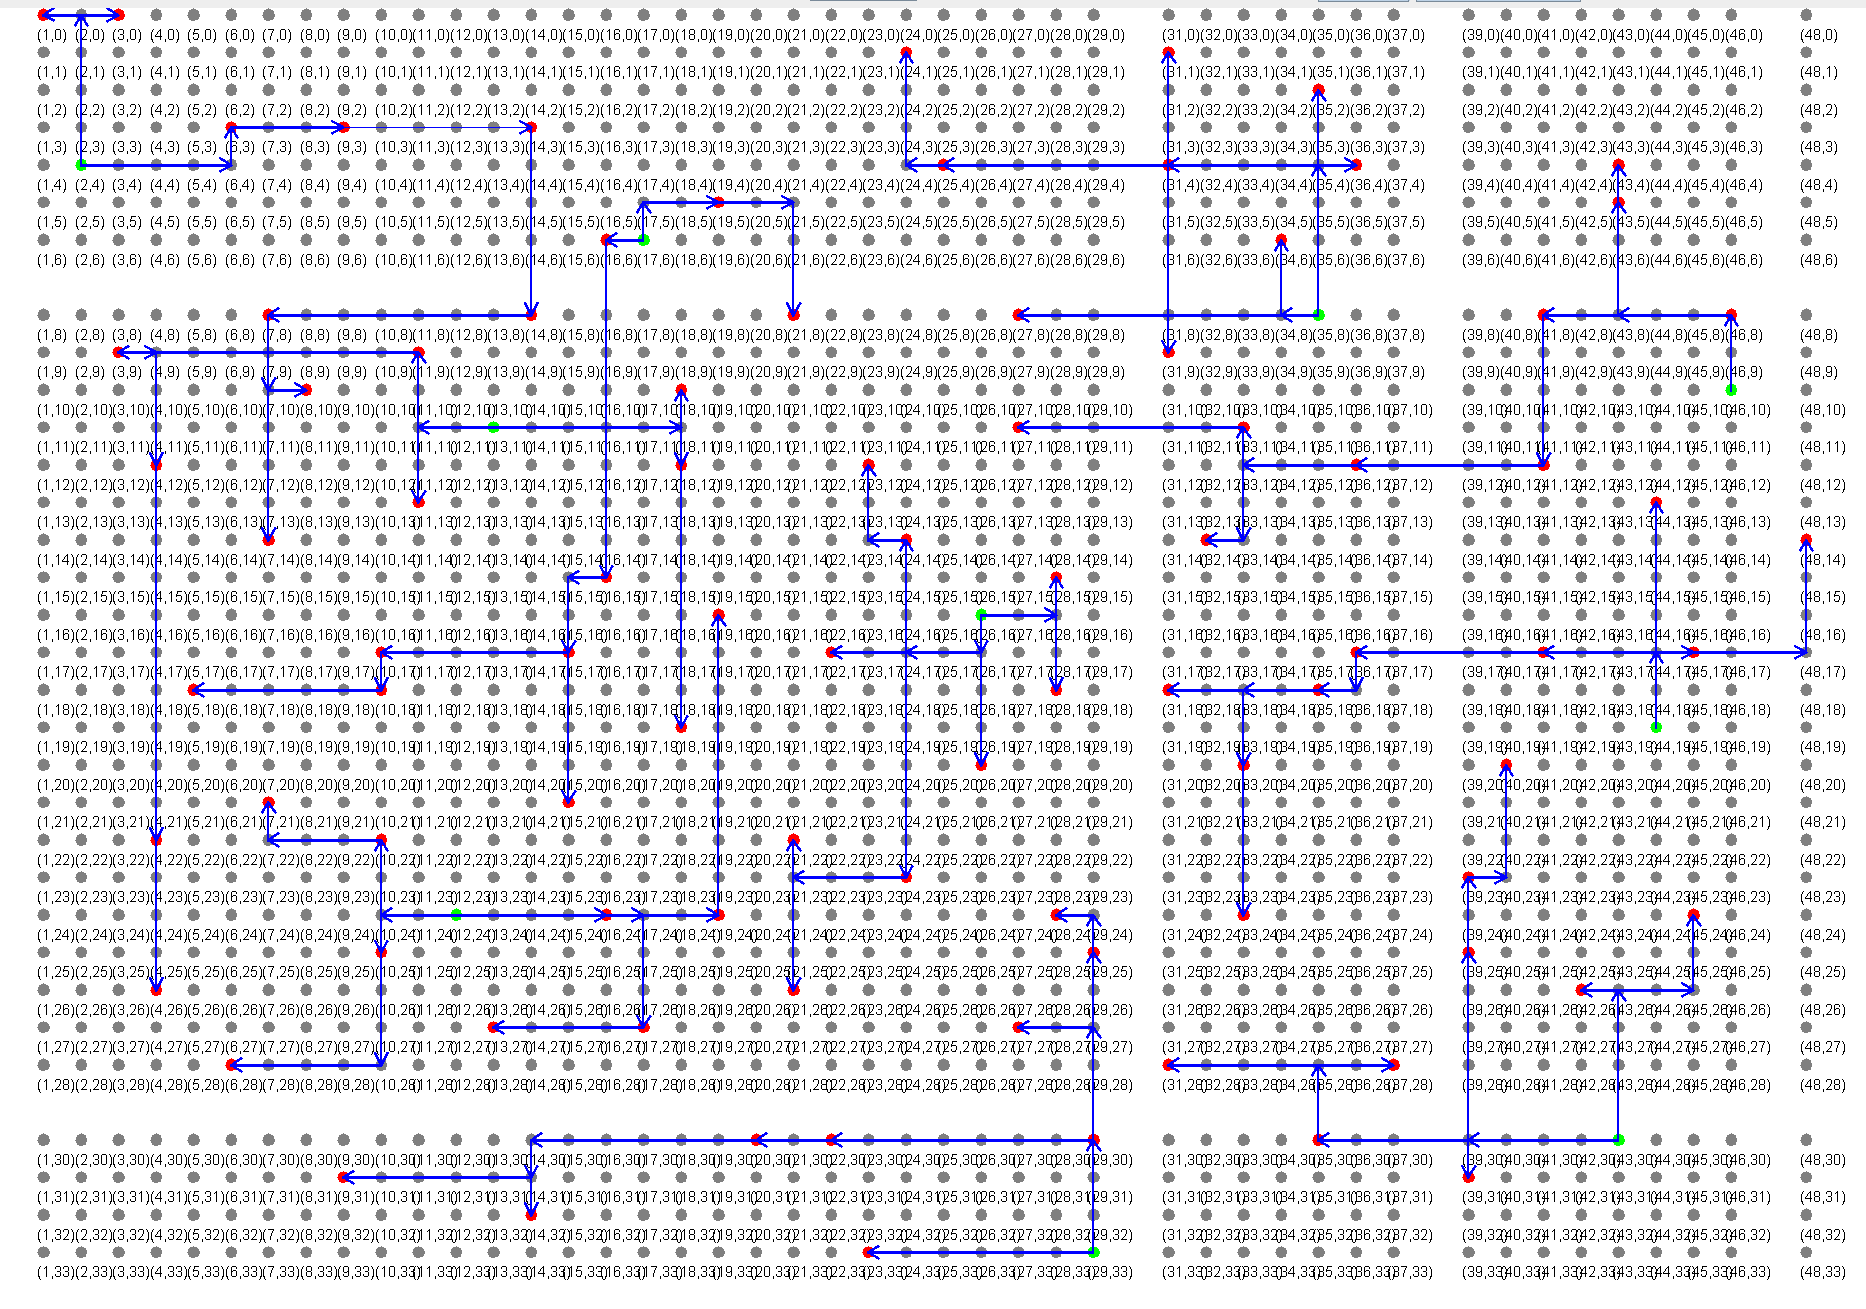
\includegraphics[width=0.9\linewidth]{resultstest6.png}
    \caption{The results of a test case involving a hundred nodes allowed to run for twenty minutes}
    \label{fig:testcase5results}
\end{figure}

This was performed and the results were as expected, a more efficient solution was found at sixteen minutes and forty-four seconds into the runtime. While it can not be determined this was the most efficient solution, due to the algorithm still not having time to complete, this clearly shows that allowing the program to run for longer for larger input sizes will allow the optimal solution to be found. 

\subsection{Summary}
Given the results described in the above sections, it can be concluded that this solution scales very well. However, as the size of inputs becomes larger, the more time is required to be confident a solution is optimal - by allowing the optimiser to complete. With that in mind, given a non-finite amount of time, the solution can scale to solve any problem of this form.

\section{Objective Evaluation}\label{objectiveeval}
This section will determine if the project was successful by comparison against the objectives defined in Section \ref{objectives}.

\begin{enumerate}
    \item Objective one was to "Research and identify how water distribution systems function". This was performed in Section \ref{waterdistributionsystems} and as such this objective was met.
    \item Objective two was to "Research optimisers and choose an optimiser to use". This was performed as outlined in Section \ref{evaluationofsolvers} and it was determined Gurobi would be the best optimiser for the given task.
    \item Objective three was to "Devise a list of functional and non-functional requirements for the theorised application". This was also performed and a full list of functional, non-functional, and optional requirements were devised as outlined in Section \ref{systemrequirements}.
    \item Objective four was to "Produce a mathematical formulation of the problem". This was performed as outlined in Chapter \ref{Modelling} and a valid mathematical formulation to solve the given problem was formulated.
    \item Objective five was to "create any classes that may be required". This was performed as outlined in Section \ref{classes}.
    \item Objective six was to "Create a GUI that allows the new classes and features to be viewed". This was performed as outlined in Section \ref{gui}.
    \item Objective seven was to "implement the mathematical formulation in to the optimiser as a series of constraints". This was performed as outlined in Section \ref{solver}.
    \item Objective eight was to "iteratively refine the algorithm based on test results, ensuring that it consistently produces valid and optimal solutions, ensuring to update the algorithms appropriately to fix any errors or edge cases". This was performed as outlined in Chapters \ref{Modelling} and \ref{implementation}
\end{enumerate}

\section{Function Evaluation}\label{functioneval}
This section will determine if the project was successful by comparison against the Functional Requirements, Non-Functional Requirements and Optional Requirements as outlined in Section \ref{systemrequirements}. The Result column presents the evaluation of each requirement. If the condition was completely met, the column will contain a "PASS". If the condition was only partly met, the column will contain a "PARTLY".  If the condition was not met at all, the column will contain a "FAIL".
\subsection{Evaluation of Functional Requirements}

\begin{longtable}{l p{12cm} l}
\caption{Functional Testing}\label{table:functionaltesting} \\
\toprule
ID & Requirement & Result \\
\midrule
\endfirsthead

\multicolumn{3}{c}{{\bfseries \tablename\ \thetable{} -- continued from previous page}} \\
\toprule
ID & Requirement & Result\\
\midrule
\endhead

\midrule \multicolumn{3}{r}{{Continued on next page}} \\
\endfoot

\bottomrule
\endlastfoot

\multicolumn{3}{c}{\textbf{Node Placement}} \\
FR1 & The application shall allow the user to place nodes where they wish & PASS \\
FR2 & The type of node placed shall be able to be determined at the time of placement & PASS \\

\midrule
\multicolumn{3}{c}{\textbf{Node Data Management}} \\
FR3 & The application shall store all placed nodes in memory, potentially in a list of all nodes, along with the necessary data for each node & PASS \\
FR4 & Each building node shall store a required flow demand value & PASS \\
FR5 & Each source node shall store a maximum output supply value & PASS \\

\midrule
\multicolumn{3}{c}{\textbf{Optimisation}} \\
FR6 & The application shall include a button to start the optimisation process & PASS \\
FR7 & The optimisation shall determine a valid piping configuration from sources to buildings, minimising total costs under given constraints & PASS \\

\midrule
\multicolumn{3}{c}{\textbf{Optimisation Constraints}} \\
FR8 & The optimisation shall enforce relevant network constraints, such as pipe capacity and pressure limits & PASS \\

\midrule
\multicolumn{3}{c}{\textbf{Flow Network Modelling}} \\
FR9 & Pipes shall only connect nodes that are parallel with one another & PASS \\
FR10 & Each pipe shall be unidirectional — no bidirectional flow & PASS \\
FR11 & The optimisation model shall satisfy flow conservation at all nodes and enforce demand/supply constraints & PASS \\

\midrule
\multicolumn{3}{c}{\textbf{Visual Feedback}} \\
FR12 & After optimisation, the canvas shall visually display the selected piping connections using lines between connected nodes & PASS \\
FR13 & The UI shall be automatically refreshed as optimisation results are available & PASS \\
\end{longtable}

In Section \ref{optionalrequirements}, Optional Functional Requirements were also outlined.

\begin{longtable}{l p{12cm} l}
\caption{Optional Testing}\label{table:optionaltesting} \\
\toprule
ID & Requirement & Result\\
\midrule
\endfirsthead

\multicolumn{3}{c}{{\bfseries \tablename\ \thetable{} -- continued from previous page}} \\
\toprule
ID & Requirement & Result\\
\midrule
\endhead

\midrule \multicolumn{3}{r}{{Continued on next page}} \\
\endfoot

\bottomrule
\endlastfoot

\multicolumn{3}{c}{\textbf{The application may allow customisation of, but not limited to, the following parameters:}}\\
OFR1.1 & Pipe cost per unit of distance & PASS\\
OFR1.2 & Building Pressure Requirements & PASS\\
OFR1.3 & Source Pressure Output & PASS\\
\end{longtable}

The implemented program also allows for the customisation of the Base Pipe Cost parameter.

\subsection{Evaluation of Non-Functional Requirements}

\begin{longtable}{l p{12cm} l}
\caption{Non-Functional Testing}\label{table:nonfunctionaltesting} \\
\toprule
ID & Requirement & Result \\
\midrule
\endfirsthead

\multicolumn{3}{c}{{\bfseries \tablename\ \thetable{} -- continued from previous page}} \\
\toprule
ID & Requirement & Result\\
\midrule
\endhead

\midrule \multicolumn{3}{r}{{Continued on next page}} \\
\endfoot

\bottomrule
\endlastfoot

\multicolumn{3}{c}{\textbf{Usability}}\\
NFR1 & It should be easy to differentiate between different node types, either by colour or a label & PASS\\
NFR2 & After optimisation is complete, the application should draw the connections in a distinct colour to distinguish them from node indicators & PASS\\
NFR3 & The node selection interface should be easy to use and responsive & PASS\\
\midrule
\multicolumn{3}{c}{\textbf{Performance}}\\
NFR4 & The optimisation process shall complete within a reasonable time for small to medium-sized networks & PASS\\
NFR5 & UI Interactions, for example: node placement, shall have $\leq$ 100ms latency to ensure responsiveness & PASS\\
\midrule
\multicolumn{3}{c}{\textbf{Scalability}}\\
NFR6 & The application shall support increasing number of nodes without significant UI performance degradation & PASS\\
NFR7 & Optimisation logic shall be designed to handle any given connectivity layout and large problem sizes with minimal bottlenecks & PASS\\
\midrule
\multicolumn{3}{c}{\textbf{Reliability}}\\
NFR8 & The application shall not crash or hang during UI interaction or while optimisation is in progress & PASS\\
NFR9 & The optimisation thread shall run independently from the UI to prevent freezing or blocking the interface & PASS\\
\midrule
\multicolumn{3}{c}{\textbf{Maintainability}}\\
NFR10 & The code shall be modular and separated into logical components & PARTLY\\
\midrule
\multicolumn{3}{c}{\textbf{Portability}}\\
NFR11 & The application shall run on any Java-compatible OS with Gurobi installed and licensed & PASS\\
\end{longtable}


